%% entwurf.tex
%% $Id: entwurf.tex 61 2012-05-03 13:58:03Z bless $
%%

\chapter{Conceptual Design and Implementation}
\label{ch:Conceptual Design}
%% ==============================
\par{
Without further ado, design and implementation of the initial ideas began. As Section \ref{ch:Analysis} showed, there are some potentially promising improvements to be made to run length encoding, but how well they scale and work on a larger input with versatile symbols or bytes has to be determined.
}
%% ==============================
\section{Preprocessing}
%% ==============================
\label{ch:Conceptual Design:sec:Preprocessing}

%% ==============================
\subsection{Vertical Byte Reading}
%% ==============================
\label{ch:Conceptual Design:sec:Parallel Byte Reading}
\par{
Implementing the vertical reading of the input shown in Section \ref{ch:Conceptual Design:sec:Parallel Byte Reading} was not hard but it should be kept in mind that the size of the input chunks has to be divisible by the size of 8. Otherwise parsing it into an Array of Bytes results in the last Byte having some padding which might cause problems later on.  By collecting the bits into a proprietary data structure, we avoid this problem but working with bytes internally should be easier. For larger files it should also be possible to work in space and writing the output on the fly during the reading process. Nonetheless both ways of collecting all bits of identical significance and writing on the fly are implemented.}

\subsubsection{First Ideas}
\par{
Initially some other ideas have been followed with very poor results. One idea was arranging all input bits in a Matrix or square Matrix in a way it would still be receivable later on. This way other methods from linear algebra would have been applicable to the input data, so that the construction of a triangular matrix or other preprocessing would result in long runs of zeros. Difficulties in the construction and transformation of the Data lead to the abandonment of this approach and the already described vertical interpretation was used further on.}

\subsubsection{Other Difficulties}
\par{
Other difficulties arose while performing bit operations, because it became slow on larger workloads. \\

TODO: explain used \href{https://discuss.kotlinlang.org/t/i-o-streams-for-kotlin/9802}{lib}}

\subsubsection{Compression improvements trough vertical reading}
\par{
First results of just plain binary RLE on the vertical interpretation improved its overall performance and archived a small edge over regular RLE with a reduction in the corpus size of around 3\% with 2 bits per run. 
\begin{table}[H]
	\centering
	\begin{tabular}{r|r|r}	
		bits per rle number & ratio in \% & bits per symbol in $\frac{bits}{symbol}$\\
		\hline
		3 & 110.82585915202825 & 8.86606873216226\\
		2 & 97.14322771462668 & 7.771458217170134 \\
	\end{tabular}
	\caption{Binary RLE on vertical interpreted data}
	\label{tab:t30 binary RLE on vertical interpreted data}
\end{table}
}

\par{
If we take a closer look on each file, we see similar results compared to the original proposed binary RLE, where most files had a compression ratio of around 1 with 2 bits per RLE encoded number, except for the file \textit{pic}. Average sizes are increasing again with more bits per run up to 2.5 times its original size and also the file \textit{pic} has the best compression ratio. This time although it is at its peak using 5 bits per RLE run and only archives a compression of 3.67 $\frac{bits}{symbol}$ compared to 1.56 $\frac{bits}{symbol}$ with simple binary RLE.

\begin{table}[H]
	\centering
	\begin{tabular}{r|r|r|r|r}	
		file & size original & size encoded & ratio in \% & $\frac{bits}{symbol}$\\
		\hline
		bib & 111261 & 117287 & 105.41 & 8.43\\
		book1 & 768771 & 781773 & 101.69 & 8.13 \\
		book2 & 610856 & 621173 & 101.68 & 8.13\\
		geo & 102400 & 105454 & 102.98 & 8.23\\
		news & 377109 & 377779 & 100.17 & 8.01\\
		obj1 & 21504 & 22003 & 102.32 & 8.18\\
		obj2& 246814 & 265075 & 107.39 & 8.59\\		 
		paper1 & 53161 & 54118 & 101.80 & 8.14\\		 
		paper2& 82199 & 83467 & 101.54 & 8.12\\		 
		pic & 513216 & 375791 & 73.22 & 5.85\\		 
		progc & 39611 & 38896 & 98.19 & 7.85\\		 
		progl & 71646 & 68428 & 95.50 & 7.64\\		 
		progp & 49379 & 48629 & 98.48 & 7.87\\		 
		trans & 93695 & 91883 & 98.06 & 7.84\\
		\hline
		all files & 3145718 & 3055852 & 97.14 & 7.77
	\end{tabular}
	\caption{Calgary Corpus encoded with vertical reading and 2 bits per RLE run}
	\label{tab:t41 Calgary Corpus encoded with vertical reading and 2 bits per RLE run}
\end{table}	
}
\par{
These results were already better than the simple binary RLE but they were still quite far from the expected outcome. This mainly arose because increasing the bits per run improved the result for the most significant bits but also degraded the results for the other bits. So the idea of encoding the bits of different significance with different RLE schemes with varying bits per run.  
}

\subsection{Varying maximum run lengths}
\par{
This time the most significant bits have been encoded with more bits per run than the other ones and after bench marking every combination, it turned out, with 2 bits per run and 5 bits per run for higher bits, it improved by another 4 percent. Now most files have a $\frac{bits}{symbol}$ ratio below 8, more specifically all textual files, which relates to the earlier mentioned ASCII fragments in UTF-8 encoding. This time higher possible runs on this position resulted in fewer runs in total, so in a better compression overall.
\begin{table}[H]
	\centering
	\begin{tabular}{r|r|r|r|r}	
		file & size original & size encoded & ratio in \% & $\frac{bits}{symbol}$\\
		\hline
		bib & 111261 & 110258 & 99.09 & 7.92\\
		book1 & 768771 & 733208 & 95.37 & 7.62 \\
		book2 & 610856 & 582583 & 95.37 & 7.62\\
		geo & 102400 & 121496 & 118.64 & 9.49\\
		news & 377109 & 353955 & 93.86 & 7.50\\
		obj1 & 21504 & 24067 & 111.91 & 8.95\\
		obj2& 246814 & 292143 & 118.36 & 9.46\\		 
		paper1 & 53161 & 50758 & 95.47 & 7.63\\		 
		paper2& 82199 & 78273 & 95.22 & 7.61\\		 
		pic & 513216 & 356712 & 69.50 & 5.56\\		 
		progc & 39611 & 36392 & 91.87 & 7.34\\		 
		progl & 71646 & 63902 & 89.19 & 7.13\\		 
		progp & 49379 & 45508 & 92.16 & 7.37\\		 
		trans & 93695 & 85964 & 91.74 & 7.33\\
		\hline
		all files & 3145718 & 2939315 & 93.43 & 7.47
	\end{tabular}
	\caption{Calgary Corpus encoded with vertical reading and 2 bits per RLE run and 5 for higher significance bits}
\label{tab:t42 Calgary Corpus encoded with vertical reading and 2 bits per RLE run and 5 for higher significance bits}
\end{table}
}
\par{
Applying this increase to more than the most significant bit lead to a decrease in performance, which most likely related to the shorter runs on lower order bits, seen in Section \ref{ch:Analysis:sec:Improvements by Preprocessing:subSec:vertReading}. Therefore the concept of mapping the input to lower value bytes to artificially increase runs of consecutive zeros on more significant bits had do be applied first.
}

\subsection{Byte remapping}
\par{
As shown in Section \ref{ch:Analysis:sec:Improvements by Preprocessing:subSec:byteRemapping} this effect could become useful if it resulted in longer runs. This effect was also seen in the second and third most significant bit, as higher value bytes became unlikely in the input data after the remapping so the idea of varying maximum run lengths for different significant bits became more appealing again. To determine the best combination of maximum run lengths and how many most significant bits should be encoded with a higher maximum run length, all combinations of these were tested and the results plotted below.
}

TODO: fix plot scaling

\begin{figure}[H]
%\begin{scaletikzpicturetowidth}{\textwidth}
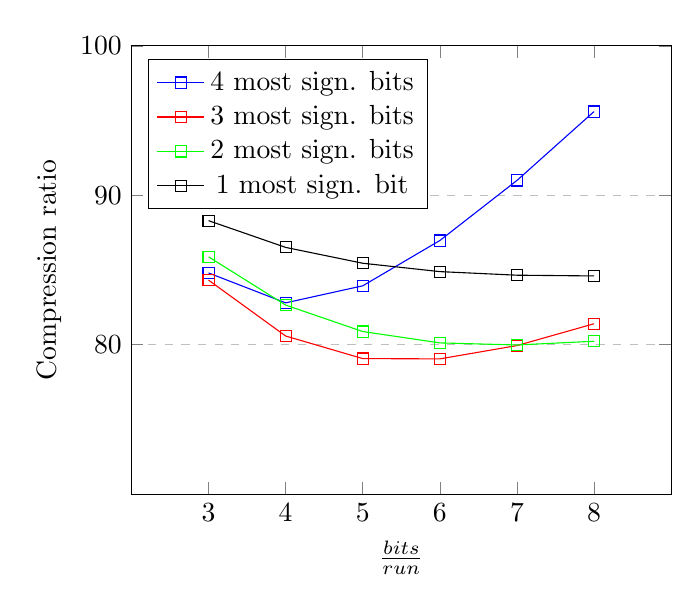
\begin{tikzpicture}%[scale=\tikzscale]
\begin{axis}[
xlabel={$\frac{bits}{run}$},
ylabel={Compression ratio},
xmin=2, xmax=9,
ymin=70, ymax=100,
xtick={3,4,5,6,7,8},
ytick={80,90,100},
legend pos=north west,
ymajorgrids=true,
grid style=dashed,
]
\addplot[
	color=blue,
	mark=square,
	]
	coordinates {
		(3,84.80)(4,82.80)(5,83.94)(6,86.97)(7,90.99)(8,95.60)
	};
\addplot[
	color=red,
	mark=square,
	]
	coordinates {
		(3,84.32)(4,80.58)(5,79.07)(6,79.05)(7,79.94)(8,81.40)
	};
\addplot[
	color=green,
	mark=square,
	]
	coordinates {
		(3,85.88)(4,82.65)(5,80.88)(6,80.12)(7,79.98)(8,80.23)
	};
\addplot[
	color=black,
	mark=square,
	]
	coordinates {
		(3,88.30)(4,86.51)(5,85.45)(6,84.89)(7,84.65)(8,84.60)
	};
	\legend{4 most sign. bits,3 most sign. bits,2 most sign. bits, 1 most sign. bit}
\end{axis}
\end{tikzpicture}
%\end{scaletikzpicturetowidth}
\caption{Different run lengths for byte mapping and varying maximum run lengths}
\label{fig:2:different run lengths for byte mapping and varying maximum run lengths}
\end{figure}

\par{
Empirically, the combination of 2 bits per run and 5 bits per run for the 3 most significant bits yielded the overall best results with 79\% of its original size and 6.32 $\frac{bits}{symbol}$. It has to be mentioned, that the expected overhead is rather small but the increase in average run length lead to a reduction in size.

\begin{table}[H]
	\centering
	\begin{tabular}{r|r|r|r|r}	
		file & size original & size encoded & ratio in \% & $\frac{bits}{symbol}$\\
		\hline
		bib & 111261 & 97867 & 87.96 & 7.03\\
		book1 & 768771 & 579649 & 75.39 & 6.03 \\
		book2 & 610856 & 484989 & 79.39 & 6.35\\
		geo & 102400 & 116487 & 113.75 & 9.10\\
		news & 377109 & 315446 & 83.64 & 6.69\\
		obj1 & 21504 & 23871 & 111.00 & 8.88\\
		obj2& 246814 & 276301 & 111.94 & 8.95\\		 
		paper1 & 53161 & 43556 & 81.93 & 6.55\\		 
		paper2& 82199 & 62544 & 76.08 & 6.08\\		 
		pic & 513216 & 272034 & 53.00 & 4.24\\		 
		progc & 39611 & 33073 & 83.49 & 6.67\\		 
		progl & 71646 & 53653 & 74.88 & 5.99\\		 
		progp & 49379 & 39400 & 79.79 & 6.38\\		 
		trans & 93695 & 84494 & 90.17 & 7.21\\
		\hline
		all files & 3145718 & 2487460 & 79.07 & 6.32
	\end{tabular}
	\caption{Calgary Corpus encoded with vertical reading, byte remapping and 2 bits per RLE run and 5 for the 3 most significance bits}
\label{tab:t43 Calgary Corpus encoded with vertical reading, byte remapping and 2 bits per RLE run and 5 for the 3 most significance bits}
\end{table}
}

\subsection{Burrows-Wheeler-Transformation Appliance}
\par{
Another possible preprocessing step which promised an improvement is the mentioned Burrows-Wheeler-Transformation from Section \ref{ch:Principles of compression:sec:Other:subSec:bwt}, initially applied to regular binary and byte wise RLE. By mistake a very simple transformation implementation was chosen, working by adding additional start and stop symbols to the input string (0x02 as STX, start of text and 0x03 as ETX, end of text). Some basic testing and playing around worked great but later on it revealed some major issues. For example the Calgary Corpus consists of more than textual data, in fact the files geo, obj1, obj2 and pic contain of some binary data of include the symbols STX or ETX so we wont be able to apply the transformation to these. Another shortcoming was the very poor time complexity of almost $O (n^2)$ because under the hood, it uses a dual pivot Quick-sort algorithm from the JDK 11, which is typically faster than traditional one pivot Quick-sort. This algorithm offers $\Theta (n \: log(n))$ average time complexity but in the worst case, its time complexity is cubic. This problem was partially solved by reading the input data in parts and performing the transformation on each part, result in a much smaller length $n$ and thus better run time at the expense of a slightly worse transformation result. As all chunks are individual transformations, they can also be computed in parallel without much effort.

\begin{table}[H]
	\centering
	\begin{tabular}{r|r|r}	
		bits per rle number & ratio in \% & bits per symbol in $\frac{bits}{symbol}$\\
		\hline
		3 & 95.4169856525027 & 7.633358852200216\\
		2 & 91.391 & 7.311309412577118 \\
	\end{tabular}
	\caption{Initial BWT implementation on byte wise RLE}
	\label{tab:t11 Simple Burrows Wheeler Transformation on byte wise RLE}
\end{table}
}
\par{
While it was only applicable to textual data and very slow, even when divided into smaller parts and computed in parallel, it improved the overall results of byte wise RLE by 16\% to a compression ratio of slightly over 7 $\frac{bits}{symbol}$ which seemed like a good start. Regular binary RLE did not really benefit from this transformation as expected but on vertical interpretation, consecutive characters result in successive bits on every significance. Still this implementation had to be dropped and switched against one that could handy arbitrary input to be able to transform all files. This time all files could be processed and the resulting compression with byte wise RLE improved further.

\begin{table}[H]
	\centering
	\begin{tabular}{r|r|r}	
		bits per rle number & ratio in \% & bits per symbol in $\frac{bits}{symbol}$\\
		\hline
		3 & 91.62970107301417 & 7.3303760858411335\\
		2 & 89.46313687368035 & 7.157050949894428
	\end{tabular}
	\caption{Burrows Wheeler Transformation on byte wise RLE}
	\label{tab:t12 Burrows Wheeler Transformation on byte wise RLE}
\end{table}
}

\par{
In Section \ref{ch:Principles of compression:sec:Other} the Burrows-Wheeler-Transformation inversion was performed using a Matrix M containing all cyclic rotations of the input word, sorted in lexicographic order. However this is has a bad complexity and the inverting process does not even has access to this Matrix M.\\

TODO: explain creation using suffix array \\

TODO: create inversion using Lyndon words\\
}

\par{
In general a Burrows-Wheeler-Transformation should also increase the runs in the implementation of Section \ref{ch:Conceptual Design:sec:Parallel Byte Reading} and \ref{ch:Analysis:sec:Improvements by Preprocessing:subSec:byteRemapping} so those preprocessing steps were also applied in combination.
}

%% ==============================
\section{Other Processing Options}
%% ==============================
\label{ch:Conceptual Design:sec:Postprocessing}
- encoding with huffman codes\\
\ldots

\subsection{Performance improvements}

%% ==============================
\section{Implementation Decisions}
%% ==============================
\label{ch:Conceptual Design:sec:Implementation Decisions}
- why kotlin\\
- performance improvements with the graalvm\\
- other decisions\\
\ldots

%% ==============================
\section{Implementation Detail}
%% ==============================
\label{ch:Conceptual Design:sec:Implementation Detail}
- detailed information about specific modules and classes\\
\ldots

\subsection{Burrows Wheeler Transformation}
- TBD\\
\subsection{Byte Remapping}
- show use case \\

%% ==============================
\section{Implementation Evaluation}
%% ==============================
\label{ch:Conceptual Design:sec:Implementation Evaluation}
- evaluation of implementation choices made


%% ==============================
\section{Summary}
%% ==============================
\label{ch:Conceptual Design:sec:Summary}

Am Ende sollten ggf. die wichtigsten Ergebnisse nochmal in \emph{einem}
kurzen Absatz zusammengefasst werden.

%%% Local Variables: 
%%% mode: latex
%%% TeX-master: "thesis"
%%% End: 
